\documentclass[11pt]{article}
\usepackage[english]{babel}
\usepackage{array} % for better arrays (eg matrices) in maths
\usepackage{booktabs} %Tablas quedan mejor
\usepackage{vmargin} %M�rgenes
\usepackage{hyperref}
\setpapersize{A4}
\setmargins{2.5cm}       % margen izquierdo
{1.5cm}                        % margen superior
{16.5cm}                      % anchura del texto
{22.42cm}                    % altura del texto
{10pt}                           % altura de los encabezados
{1.5cm}                           % espacio entre el texto y los encabezados
{0pt}                             % altura del pie de p�gina
{2cm}                           % espacio entre el texto y el pie de p�gina

\usepackage[none]{hyphenat} %No corta palabras al final de las lineas
\usepackage{graphicx} %Im�genes
\usepackage{subfigure} % subfiguras
\graphicspath{{img/}} % Root for images
\usepackage{wrapfig}
\usepackage{siunitx} %Escribir n�meros y unidades
\usepackage{amsmath} %Mayor facilidad para escribir matrices y otros elementos matem�ticos
%\numberwithin{equation}{section} %En las ecuaciones se especifica tambi�n el cap�tulo
\usepackage{xcolor} %Colores (\color{})
\usepackage{lipsum}
\usepackage{topcapt}
\usepackage{parskip}
\usepackage{braket}
\usepackage{setspace}
\usepackage{listings}
\usepackage{fancyhdr} %Cabeceras
\pagestyle{fancy} % seleccionamos un estilo


\lhead{C programming and performance} %CAMBIA
\rhead{Parallel programming} %CAMBIA





\begin{document}

\setstretch{1.5} % Line spacing of 1.5
\setlength{\parskip}{5mm}

\renewcommand{\tablename}{Table}

\thispagestyle{empty} %Primera p�gina sin n�mero
\begin{center}
	
	{\scshape\LARGE Parallel programming\par}
	\vspace{0.5cm}
	\rule{15cm}{0.8pt}\\
	{\huge\bfseries C programming and performance: N-body\par}
	\rule{15cm}{0.8pt}\\
	\vspace{0.5cm}
	{\large \itshape Jorge Pardillos, Michal Kustosz\par}

\end{center}
\setcounter{page}{1} %Empezamos a contar los n�meros



\pagenumbering{arabic} %Ponemos n�meros normales (�rabes) ya
\pagestyle{fancy} % seleccionamos un estilo


\section{Introduction}

The subject of this report is analysis of a program solving \emph{N-body} problem. This is done by a step-by-step simulation of celestial bodies in discrete time.
Our objective is to understand the complexity of the code, the way the compiler works and also how it's executed by the machine. Also the task is to perform optimisations by changing the code or by vectorisation using SIMD architecture.

\section{Complexity of the algorithm}

We start working with the baseline program that has been provided. Our first goal will be to perform an initial analysis on the code, finding which ``operation'' is the basic one of the program. It is trivial to se that the main part of the code is the following one:

\begin{lstlisting}
for t = 0 to MAX_TIME
    for i = 0 to N
        for j = 0 to N
	      force[i] += bodyBodyInteraction(pos[i], pos[j]);
    for i = 0 to N
        pos[i], vel[i] = advance_step(pos[i], vel[i], force[i], dt);
\end{lstlisting}


In the code above there are two basic operations. The first one computes the new force acting on the body \emph{i}, we are computing this force N times for each body, so that leaves us with a total of $N^2$ operations for the body-body interaction. The second operation is updating the velocities, positions and forces for each body, but we are doing this operation N times, so the dominant operation will be the \emph{body-body interaction}, and the overall complexity is about $N^2$. In the big-O notation the complexity is
\begin{equation*}
\mathcal{O}(N^2+N) = \mathcal{O}(N^2)
\end{equation*}

\section{Baseline program}

The next step consists of studying the effect of the size of the problem on it's execution time and metrics. These are the metric results for the given size and iterations of the code:
\begin{table}[htbp]
\centering
\begin{tabular}{l c c c c c c c c r}
\toprule

N	&	Cycles	&	GHz	&	Insns	&  Insns/cycle	&	cache-misses & Seconds	\\												
\midrule
20000 &  398.382.665.850 & 3,244 & 560.581.340.117 & 1,41 & 323.472 & 124,9973\\
2000 & 3.621.480.028 & 3,238 &  5.622.625.091 & 1,55 & 5.100 & 1,1731\\
200 & 38.762.207 & 3,237 & 58.785.447 & 1,52 &  1.899 & 0,0896\\
20 & 1.670.067 & 3,215 & 1.657.107 & 0,99 & 1.582 & 0,1020\\
\bottomrule							
\label{table:Baseline_gcc}
\end{tabular}
\caption{Metric results for the baseline program depending on size, for $t=100$. Compiler: gcc 6.1.0. $3.30$GHz}
\end{table}

In order to compare results, we can make the same simulations with the Intel C compiler (icc\,16.0.0). These are the results:
\begin{table}[htbp]
\centering
\begin{tabular}{l c c c c c c c c r}
\toprule

N	&	Cycles	&	GHz	&	Insns	&  Insns/cycle	&	cache-misses & Seconds	\\												
\midrule
20000 &  284.315.905.359 & 3,238 & 590.428.579.963 & 2,08 & 28.741 & 87,7695\\
2000 &  2.796.167.620 & 3,238 &  5.922.750.068 & 2,12 & 5.702 & 0,9088\\
200 & 30.720.440 & 3,237 & 62.132.267 & 2,02 &  2.691 & 0,0960\\
20 & 1.978.480 & 3,219 & 2.047.869 & 1,04 & 2.143 & 0,0446\\
\bottomrule							
\label{table:Baseline_icc}
\end{tabular}
\caption{Metric results for the baseline program depending on size, for $t=100$. Compiler: intel 16.0.0. $3.30$GHz}
\end{table}

\newpage

Now we can compare both compilers depending on execution time and size of the problem, for example (due to the huge differences the graph is represented in logarithmic scale):
\begin{figure}[htbp] %  figure placement: here, top, bottom, or page
   \centering
   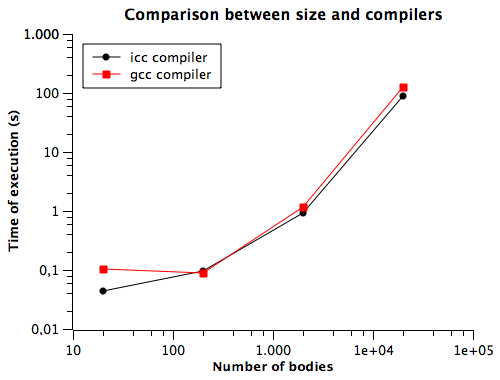
\includegraphics[width=4in]{compilers.png} 
   \caption{Effect of compilers and size}
   \label{fig:example}
\end{figure}

In the previous image it is clear that the problem has an order $N^2$.

Analysing the basic aspects of the baseline program, we can try to see the difference of implementing an optimisation option in the compiling phase and just compiling the code without any other special order. For example for the gcc compiler these are the results obtained:

\begin{table}[htbp]
\centering
\begin{tabular}{l c c c c c c c c r}
\toprule

N	&	Cycles	&	GHz	&	Insns	&  Insns/cycle	&	cache-misses & Seconds	\\												
\midrule
2000 & 164.488.050.082 & 3,346 &  162.823.986.804 & 0,99 & 1.815.045 & 49,1090\\
200 & 1.645.949.655 & 3,222 & 1.634.022.701 & 0,99 & 2.832  & 0,5318\\
20 & 18.098.698 & 2,561 & 17.919.614 & 0,99 & 1.768 &0,0951\\
\bottomrule							
\label{table:Baseline_NotOpt}
\end{tabular}
\caption{Metric results for the baseline program (not optimised) depending on size, for $t=100$. Compiler: gcc 6.1.0. $3.30$ GHz}
\end{table}

\newpage

Comparing the table \ref{table:Baseline_Slow} and the first one it is possible to see that there are huge differences between both performances, the execution time for the last one is quite higher than the optimised code (the execution for N=20000 bodies has not been done due to its long execution time), the instructions are much more but the cycles are even more, so rate of cycles per cycle is much lower in the not optimised program. It is clear that it is more efficient in all aspects to execute an optimised code.


At the same time, if we do not execute the loop of the main function and execute the code, we can see how long does it take to initialise the variables in each scenario. We can see that, for example with the \emph{gcc -Ofast} compiler, we get the following results:
\begin{table}[htbp]
\centering
\begin{tabular}{c c c c c}
\toprule

N & 20000	&	2000	&	200	&	20	\\												
\midrule
Whole code (s) & 124,9973 & 1,1731 & 0,0896 & 0,1020\\
Initialisation (s) & 0,0029 & 0,0012 & 0,0009 & 0,0012\\
\% & 0,00232 & 0,102 & 1,004 & 1,176\\
\bottomrule							
\label{table:Baseline_Percent}
\end{tabular}
\caption{Importance of initialisation phase depending on size. Compiler: gcc 6.1.0. $3.30$ GHz}
\end{table}

It is clear that as the size of the problem is bigger and bigger, the initialisation steps are not going to be the relevant part of the function.

\section{Optimisation and vectorisation}

The first obvious idea (which has already been done) is to define what type of variables should we use (\emph{double} or \emph{float}). In our previous executions we have used floats, adding the option \emph{-DFP32=1} in the compiling phase, which implies working with float variables, thus using less memory for the allocation of variables and making the program faster. If otherwise we had used the option \emph{-DFP64=1} or omitted this option, we would have been working with doubles instead of floats, using more memory (the double) than we needed, and making the execution much slower.

The following results are obtained when the program uses doubles:

\begin{table}[htbp]
\centering
\begin{tabular}{l c c c c c c c c r}
\toprule

N	&	Cycles	&	Instructions	&  Insns/cycle & task-clock	&	cache-misses & Seconds	\\												
\midrule
20000 & 1.134.251.737.654 & 901.314.182.517  & 0,79 & 343468,98 & 18.164.701 & 343,1313\\
2000 & 11.326.683.507 & 9.031.391.827  & 0,80 & 3498,80 &612.784  & 3,5591\\
200 & 115.651.379 & 93.037.618 & 0,80 & 35,731358 & 14.309 & 0,0397\\
20 & 2.831.749 & 2.025.708 & 0,72& 0,880500 & 6.975 & 0,054987507\\
\bottomrule							
\label{table:Baseline_Slow}
\end{tabular}
\caption{Metric results using doubles, for $t=100$. Compiler: gcc 6.1.0. $3.30$GHz}
\end{table}


In order to compare the results, the performance will be expressed as \emph{Work/second}:
\begin{gather*}
P=\frac{W}{s}=\frac{\text{operations}}{\text{instruction}}\frac{\text{instructions}}{\text{cycle}}\frac{\text{clock cycles}}{\text{second}}\\
P=\frac{N^2*\emph{iter}}{\text{instructions}}\frac{\text{instructions}}{\text{cycles}}\frac{1}{330GHz}
\end{gather*}

For our implementations we will take as fixed parameter $N=2000$ bodies and $t=100$, and we will take the code that uses doubles as the baseline code. One step is equivalent to one body-body interaction.

\begin{table}[htbp]
\centering
\begin{tabular}{l c c c}
\toprule

Program & Code eficienfy	&	IPC	&  Performance\\
& (Steps/Inst) & (Steps/Inst) & (GSteps/sec)\\	
\midrule
Baseline &0,04 & 0,7946 & 0,11\\
Floats & 0,07 & 1,55 & 0,35\\
\bottomrule							
\label{table:Baseline_Double}
\end{tabular}
\caption{Metric results using doubles, for $t=100$ and $N=2000$. Compiler: gcc 6.1.0. $3.30$GHz}
\end{table}

We see that maybe we could do a \emph{loop fussion} in the core of the pogram, in the \textbf{integrate} function we could try to merge both loops in the variable \emph{i}. These are the results for this implementation:
\begin{table}[htbp]
\centering
\begin{tabular}{l c c c}
\toprule

Program & Code eficienfy	&	IPC	&  Performance\\
& (Steps/Inst) & (Steps/Inst) & (GSteps/sec)\\									
\midrule
Baseline &0,04 & 0,7946 & 0,11\\
Floats & 0,07 & 1,55 & 0,35\\
Loop fussion & 0,07 & 1,53  & 0,35\\
\bottomrule							
\label{table:LoopFussion}
\end{tabular}
\caption{Loop fussion, for $t=100$ and $N=2000$. Compiler: gcc 6.1.0. $3.30$GHz}
\end{table}

It is easy to see that it has been of no effect, the performance is exactly the same.

We could try as well to do some other optimisation the one we performed in the Laplace program, changing the roles of $A_{\text{new}}$ and $A$, but in this case it will be useless as well, because we are working with pointers, and changing them does not requiere memory.

From now on we will only work with \emph{floats} (\emph{-DFP32=1}). We have done two different optimisations, and the results will be shown on three different compilers: \emph{gcc/6.1.0}, \emph{gcc/4.8.5} and \emph{intel/16.0.0}.

The first optimisation implemented is more related with physics than programming, but still it should be taken into account. It is based on the third physical law, for every action there is a force opposite and equal in magnitude. Thus there is no need to make two separate calculations for the force caused by the body $i$ or the body $j$ and viceversa, it is possible to use the same result on both of them.

Taking into account this new approach, the main loop iterations decrease to half of the original ones, so the complexity is of the order of $N^2/2$. The results are given in the in section \ref{results}.

The second optimisation is the vectorisation of the code exploiting  the \emph{SIMD} architecture. For that reason multiple changes to the code were applied.

In first place, the representation of data had been changed: instead of arrays of points (the data was previuously saved as an array of points, and each point had spacial 3D coordinates and mass), is has been arranged as arrays of coordinates, one for each direction axis. That allowed to process one array of continuous data at the time, and vectorise it efficiently, and also avoid cache misses.

An example of the new code is given (\emph{forj} means a loop for j = i + 1 to $N$):
\begin{lstlisting}
#pragma omp simd 
forj { rxs[j] = Xin[j] - Xin[i]; }
#pragma omp simd 
forj { rys[j] = Yin[j] - Yin[i]; }
#pragma omp simd
forj { rzs[j] = Zin[j] - Zin[i]; }
\end{lstlisting}

\newpage

\section{Results}
\label{results}

We will study the effect for each one of the two main optimisations, comparing them with the baseline (using floats), in each of the compilers.

\subsection{gcc (4.8.5)}

\begin{table}[htbp]
\centering
\begin{tabular}{l c c c}
\toprule
Program & Code eficienfy	&	IPC	&  Performance\\
& (Steps/Inst) & (Steps/Inst) & (GSteps/sec)\\									
\midrule
Baseline (floats) & 0,034 & 0,861 & 0,096\\
Iteration reduction & 0,032 & 1,635 & 0,173\\
Vectorisation & 0,033 & 1,872 & 0,198\\
\bottomrule							
\label{table:GCC4}
\end{tabular}
\caption{Performance for the optimisations, for $t=100$ and $N=2000$. Compiler: gcc 4.8.5. $3.30$GHz}
\end{table}

In this case we observe an improvement over the optimisations in the IPC (instructions per cycle), while the code efficiency, the number of body-body interactions per instruction, stays invariant in all the implementations. Therefore the performance gets better and better in each implementation, as expected.


\subsection{gcc (6.1.0)}


\begin{table}[htbp]
\centering
\begin{tabular}{l c c c}
\toprule
Program & Code eficienfy	&	IPC	&  Performance\\
& (Steps/Inst) & (Steps/Inst) & (GSteps/sec)\\									
\midrule
Baseline (floats) & 0,071 & 1,541 & 0,355\\
Iteration reduction & 0,033 & 1,582 & 0,173\\
Vectorisation & 0,053 & 1,633 & 0,281\\
\bottomrule							
\label{table:GCC6}
\end{tabular}
\caption{Performance for the optimisations, for $t=100$ and $N=2000$. Compiler: gcc 6.1.0. $3.30$GHz}
\end{table}

In this case it is observed that the basic program (with the optimising option \emph{-Ofast}) already performs quite well: the code is more efficient and the performance is higher than any other value of the previous case. The IPC metric is as well quite good.

However when the optimisations are implemented it is observed that this case is worse than expected, and worse than the original program in efficiency, while the IPC stays similar, so the performance is also worse. We can only suggest that this version of the \emph{gcc} compiler does already an excellent performing job.

\subsection{intel (16.0.0)}

\begin{table}[htbp]
\centering
\begin{tabular}{l c c c}
\toprule
Program & Code eficienfy	&	IPC	&  Performance\\
& (Steps/Inst) & (Steps/Inst) & (GSteps/sec)\\									
\midrule
Baseline (floats) & 0,068 & 2,100 & 0,460\\
Iteration reduction & 0,038 & 1,569 & 0,195\\
Vectorisation & 0,114 & 2,112 & 0,782\\
\bottomrule							
\label{table:GCC6}
\end{tabular}
\caption{Performance for the optimisations, for $t=100$ and $N=2000$. Compiler: intel 16.0.0. $3.30$GHz}
\end{table}

Finally, with the Intel compiler it is visible that the original program is better than some of the previous cases. At the same time when the optimisations are implemented we find that the vectorisation is giving quite good results, improving significantly the performance, code efficiency and IPC. Processing one array at the time reduced significantly number of instructions and cycles in the program execution.

Graphs for the evolution of the three parameters have been made:

\begin{figure}[htbp] %  figure placement: here, top, bottom, or page
   \centering
   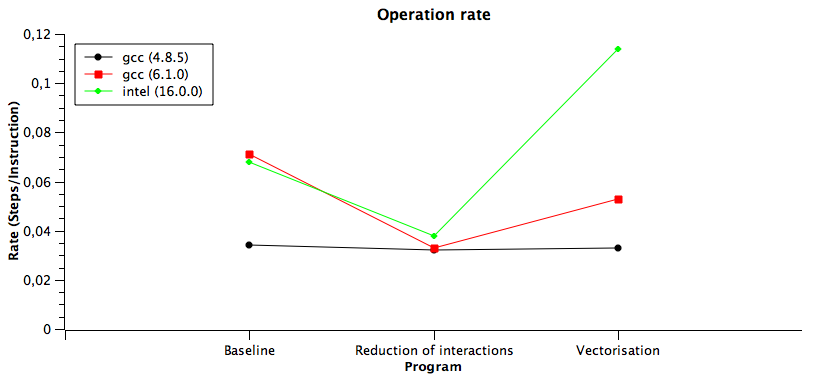
\includegraphics[width=5in]{OpRate.png} 
   \caption{Operation rate metrics}
   \label{fig:example}
\end{figure}
\begin{figure}[htbp] %  figure placement: here, top, bottom, or page
   \centering
   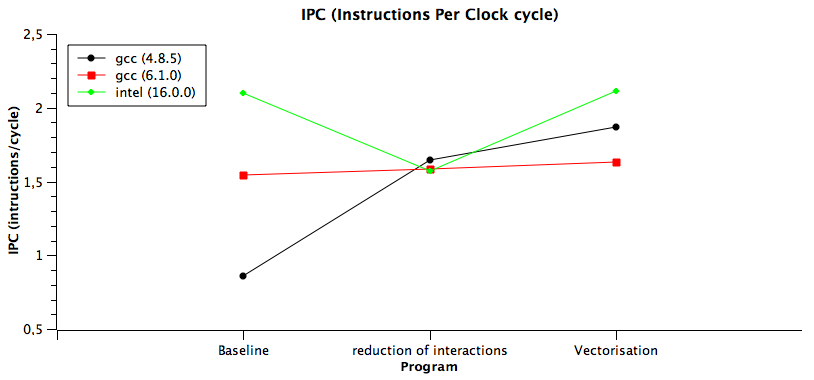
\includegraphics[width=5in]{IPC.png} 
   \caption{IPC metrics}
   \label{fig:example}
\end{figure}
\begin{figure}[htbp] %  figure placement: here, top, bottom, or page
   \centering
   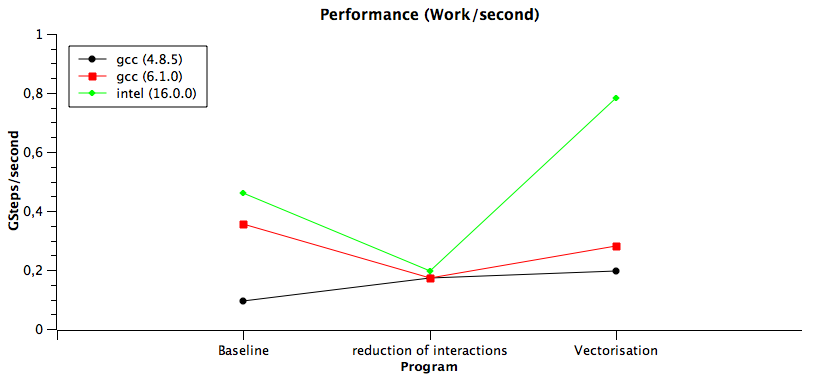
\includegraphics[width=5in]{Performance.png} 
   \caption{Performance metrics}
   \label{fig:example}
\end{figure}
\section{Summary}
The result of the task is somehow unexpected. The first thing which is unusual is that the performance of the gcc/6.1.0 decreased after optimizations. It may be that this complier with -Ofast optimisations works much better since it is not said to him how to optimise in particular. \\
The second thing to explain is the performance decrease for the two compliers based on gcc/6.1.0 after the first optimization in code. This may be due to the implementation, which during one run of the loop made two assignments to an array in different places in the memory:
\begin{lstlisting}
forceX[i] += tempXForce;
forceX[j] -= tempXForce;
\end{lstlisting}
Maybe in this case it is more reasonable to make two times more iterations, but with updating consecutive memory blocks.\\
The only success was achieved with Intel compiler after vectorizing the code. It seems that only this compiler can fully exploit the SIMD architecture of Intel processors. The performance boost after applying optimizations in code was significant.



\end{document}

























